%\documentclass{uai2021} % for initial submission
 \documentclass[accepted]{uai2021} % after acceptance, for a revised
                                    % version; also before submission to
                                    % see how the non-anonymous paper
                                    % would look like
% NOTE: Only comment/uncomment the lines above as appropriate,
%       as they will be replaced automatically for papers to be published.
%       Do not make any other change above this note for an accepted
%       version.

%% Choose your variant of English; be consistent
\usepackage[american]{babel}
% \usepackage[british]{babel}

%% Some suggested packages, as needed:
\usepackage{natbib} % has a nice set of citation styles and commands
    \bibliographystyle{plainnat}
    \renewcommand{\bibsection}{\subsubsection*{References}}
\usepackage{mathtools} % amsmath with fixes and additions
% \usepackage{siunitx} % for proper typesetting of numbers and units
\usepackage{booktabs} % commands to create good-looking tables
\usepackage{tikz} % nice language for creating drawings and diagrams

%%%%%%%%%%%%%%%%%%%%%%%%%%%

\usepackage{amsfonts}
\usepackage{amsthm}

%%%%%%%%%%%%%%%%%%%%%%%%%%%

%% Provided macros
% \smaller: Because the class footnote size is essentially LaTeX's \small,
%           redefining \footnotesize, we provide the original \footnotesize
%           using this macro.
%           (Use only sparingly, e.g., in drawings, as it is quite small.)

%% Self-defined macros
\newcommand{\swap}[3][-]{#3#1#2} % just an example


%%%%%%%%%%%%%%%%%%%%%%%%%%%

\newtheorem{thm}{Theorem}
\newtheorem{algo}[thm]{Algorithm}
\newtheorem{ass}[thm]{Assumption}
\newtheorem{cor}[thm]{Corollary}
\newtheorem{defn}[thm]{Definition}
\newtheorem{exmp}[thm]{Example}
\newtheorem{lem}[thm]{Lemma}
\newtheorem{prop}[thm]{Proposition}
\newtheorem{rem}[thm]{Remark}


\newcommand{\pa}{\textnormal{pa}}

\newcommand{\ds}{\text{ds}}
\newcommand{\dt}{\text{dt}}

\newcommand{\disjU}{\mathbin{\dot{\cup}}}

\usepackage{tikz}
\usepgflibrary{arrows}
\usetikzlibrary{shapes}
\usetikzlibrary{arrows.meta}
\usetikzlibrary{positioning}

\usepackage{graphicx}
\usepackage{caption}
\usepackage{subcaption}


%%%%%%%%%%%%%%%%%%%%%%%%%%%


\title{Equality Constraints and Causal Identification in Linear Hawkes 
Processes}

% The standard author block has changed for UAI 2021 to provide
% more space for long author lists and allow for complex affiliations
%
% All author information is authomatically removed by the class for the
% anonymous submission version of your paper, so you can already add your
% information below.
%
% Add authors in order of decreasing contribution
\author[1]{\href{mailto: Søren Wengel Mogensen 
<swemo@dtu.dk>}{Søren~Wengel~Mogensen}{}} 
% Add affiliations after the authors
\affil[1]{%
    Section of Cognitive Systems\\
    Technical University of Denmark\\
    Denmark
}

\begin{document}
\maketitle

\begin{abstract}
  This is the abstract for this article.
  It should give a self-contained single-paragraph summary of the article's contents, including context, results, and conclusions.
  Avoid citations; but if you do, you must give essentially the whole reference.
  For example: This whole paper is devoted to praising É. Š. Åland von Vèreweg's most recent book (“Utopia's government formation problems during the last millenium”, Springevier Publishers, 2016).
  Also, do not put mathematical notation and abbreviations in your abstract; be descriptive.
  So not “we solve \(x^2+A xy+y^2\), where \(A\) is an RV”, but “we solve quadratic equations in two unknowns in which a single coefficient is a random variable”.
  The reason is that mathematical notation will not display correctly when the abstract is reused on the proceedings website, for example, and that one should not assume the abstract's reader knows the abbreviation.
  Of course the same remarks hold for your paper's title.
\end{abstract}

Main focus on equality constraints: follows from parametric form of integrated 
cumulative variance matrix, biproduct: HTC-type identification results follow, 
give example of equality constraint using dynamical information (check that 
there are no equality constraints in this case using only integrated matrix)

add also injection intervention interpretation of the Hawkes processes

\section{Introduction}\label{sec:intro}

In classical work, conditional independence has been used as a testable 
implication of causal models. In addition, equality constraints (or Verma, or 
dormant, same thing?) have been proposed to distinguish between data-generating 
mechanisms. In stochastic processes, local independence is a concept which can 
be used analogous to conditional independence. In this paper, we show that one 
can also find equality constraints in the class of linear Hawkes process that 
have been a much studied model class recently in machine learning. We show that 
these class of models in a certain sense satisfy the same equality constraints 
as a cyclic linear structural equation model, and we also show that one may 
find additional constraints using when the process is observed over time.

This also naturally leads to new identification results for Hawkes processes, 
and we also give a causal interpretation of the parameters which is closely 
related to the so-called cluster representation of a linear Hawkes process.

[add that the identifiability is generic]


%%%%%%%%%%%%%%%%%%%%%%%%%%%
%%%%%%%%%%%%%%%%%%%%%%%%%%%

\section{Hawkes Processes}
\label{sec:hawPro}

\begin{defn}[Linear Hawkes process]
	We say that a point process, $N$, is a \emph{linear Hawkes process} if the 
	intensity is of the form
	
	$$
	\lambda_t^\beta = \mu_\beta + \sum_{\beta \in V} \int_{-\infty}^{t} 
	g_{\beta\alpha}(t - s) d 
	N_s^\alpha
	$$
	
	\noindent for all $\beta\in V$ and $t\in R$. 
	\label{def:hawProc}
\end{defn}

We will often refer to a linear Hawkes process by just saying Hawkes process. 
We assume throughout that $g_{\beta\alpha}$ is a continuous function for all 
$\alpha$ and $\beta$ and that the coordinate processes of the Hawkes 
process are indexed by the set $V = \{1,2,\ldots, n\}$.

We define the $n\times n$ matrix $G$ such that $G_{\beta\alpha} = 
\int_{-\infty}^\infty 
g_{\beta\alpha}(s) \ds$. We assume that the spectral radius of $G$ (largest 
absolute value of its eigenvalues) is less than 1 which implies that we can 
assume the Hawkes process to be stationary \citep{jovanovic2015}.
We define $n\times n$ matrix $R=(I_n - G)^{-1}$ where $I_n$ is the 
$n\times n$ identity matrix. This is well-defined due to the assumption on 
the spectral radius of $G$ and furthermore $R = \sum_{i=0}^\infty G^i$. 

We will introduce two statistical concepts that we will use in our results. One 
is seen to be an integrated (and time-independent) measure of covariance and 
one is seen to be a 
time-dependent measure of covariance.

The parameters in $G$ and $R$ have straightforward interpretations. From the 
definition of the Hawkes process, it follows that $G_{\beta\alpha}$ is the 
expected number of directed descendant events of type $\beta$ from an 
$\alpha$-event [make figure]. More generally, for $i = 1,2,\ldots$, 
$(G^i)_{\beta\alpha}$ is the 
expected number of $\beta$-descendants in the $i$'th generation of an 
$\alpha$-event. This implies that $R_{\beta\alpha}$ is the expected total 
number of $\beta$-descendants on an $\alpha$-tree, not counting the 
$\alpha$-root if $\alpha=\beta$. 
See also 
\cite{jovanovic2015}.
[write also as a formula, 
equation? ref, and check computation, make also sim]

%%%%%%%%%%%%%%%%%%%%%%%%%%%

\paragraph{Infinitesimal Covariance}

For a $n$-dimensional stationary point process, we define the intensity vector 
(mean vector?), following [Hawkes JRSS-B, 1971]

$$
\lambda = E(dN(t))/dt
$$

\noindent and covariance density matrix

$$
k(\tau) = 
$$

[see Hawkes JRSS-B, 1971 - compare this to bacry and muzy]
[see  Bacry and Muzy: Hawkes model for price and trades high-frequency 
dynamics, they give explanation]

%%%%%%%%%%%%%%%%%%%%%%%%%%%

\paragraph{Integrated Covariance}

We can integrate the infinitesimal covariance over time to obtain a type of 
integrated cumulant matrix, $C$. This matrix satisfies the equation

$$
C = R \Lambda R^T,
$$

see \cite{jovanovic2015}.

%%%%%%%%%%%%%%%%%%%%%%%%%%%

\paragraph{Cluster Representation}

In Definition \ref{def:hawProc}, Hawkes processes are introduced by specifying 
the intensity processes. One can also define them by using a so-called cluster 
representation which, as we will see, lends itself to a straight-forward causal 
interpretation. [this is complicated by the doubly-infinite nature of the 
process? not started at zero]

Each 
generation 0 node has an associated `Hawkes tree', i.e., the nodes that are 
descendants in the generating process (note that this is different from 
descendants in the causal graph).




%%%%%%%%%%%%%%%%%%%%%%%%%%%
%%%%%%%%%%%%%%%%%%%%%%%%%%%

\subsection{Causal Interpretation}

In this section, we will define what we mean by a {\it causal} Hawkes process. 
\cite{mogensenUAI2020} defined a causal Hawkes process by requiring that the 
set 
of functions $\{g_{\beta\alpha}\}$ also describes the influence between 
coordinate processes in intervened systems where the trajectory of some 
coordinate processes is determined exogenously. We will instead use the cluster 
representation to give a causal
interpretation based on a type of \emph{injection intervention}. That is, the 
observational state of the system is given by the Hawkes process as defined 
above. An interventional state is defined by a set of \emph{injections}, 
$\{(\alpha_i, t_i) \}_{i =1,\ldots, M} $, such that each injection is an 
element in $V\times \mathbb{R}$. [make figure to illustrate] Each injection is 
a root in a Hawkes tree and the interventional processes are given as the 
superposition of all intrinsic and interventional trees. We then say that a 
linear Hawkes process is {\it 
causal} if a Hawkes tree rooted at $\alpha$ has the same distribution as an 
intrinsic Hawkes tree for all coordinate processes $\alpha \in V$. In 
other words, the intervention events 
propagate in the same way through the system as the intrinsic events. This 
causal assumption is seen to correspond closely to 
the assumption of \emph{autonomy} or \emph{modularity} which is often used to 
define causal models 
\citep{pearl2009, petersElements2017}.

We note that this type of interventions corresponds to how interventions could 
be undertaken in some fields of 
science, e.g., in neuroscience where in some experiments on can incur a change 
in the 
action potential for some neurons, however not change their inner dynamics nor 
sever causal parents [ref]. It is also similar to how interventions are often 
modelled in control theory in which they are external forces (possibly 
dependent on the past of the process) that change the dynamics of the system 
without necessarily breaking any connections [ref].

\begin{defn}[Causal effects]
	We will say that $G_{\beta\alpha}$ is the \emph{direct (causal) effect} 
	from 
	$\alpha$ on $\beta$ and that $R_{\beta\alpha}$ is the \emph{total (causal) 
	effect} from $\alpha$ on $\beta$. We will say that $g_{\beta\alpha}$ is the 
	{\it causal function} from $\alpha$ to $\beta$.
	\label{def:cauEff}
\end{defn}

The interpretation of the entries in $G$ and $R$ (see Section 
\ref{sec:hawPro}) and the causal assumption justify the above definitions. If 
we inject an 
interventional event of type $\alpha$ at time $s \in \mathbb{R}$, this 
event on average has $G_{\beta\alpha}$ events 
of type $\beta$ as first-generation (or \emph{direct}) descendants (when 
considering all $t > s$). The Hawkes tree rooted at the 
interventional $\alpha$-event on average has a total of $R_{\beta\alpha}$ 
events of 
type $\beta$, not counting the injectional event if $\alpha=\beta$. 

%%%%%%%%%%%%%%%%%%%%%%%%%%%

\paragraph{Graphical representation}

A {\it graph} is a pair $(V,E)$ where $V$ is a finite set of nodes and $E$ is a 
set edges, each between a pair of (not necessarily distinct) nodes. We will  
consider {\it directed mixed graphs}, i.e., graphs such that every edge is 
either \emph{directed}, $\rightarrow$, or \emph{bidirected}, $\leftrightarrow$. 

Given a causal Hawkes process with coordinate processes indexed by $V = 
\{1,2,\ldots,n\}$, we construct its \emph{causal graph}, $\mathcal{D} = (V,E)$, 
such that 
$\alpha \rightarrow_\mathcal{D} \beta$ if and only if $g_{\beta\alpha} \neq 0$. 
Due 
to the assumptions of continuous and nonnegative $g_{\beta\alpha}$, we see 
that if $g_{\beta\alpha}\neq 0$, then there exist a nontrivial interval such 
that $g_{\beta\alpha} > 0$ on this interval. [is g assumed to be zero on 
negative axis?]

[introduce latent projection]


%%%%%%%%%%%%%%%%%%%%%%%%%%%
%%%%%%%%%%%%%%%%%%%%%%%%%%%

\section{Identification}

As is common [refs], our results give identification results using graphical 
constraints, i.e., sparsity as encoded by the graph.

In this paper, we will discuss the identification of the entries in the 
matrix $G$ and the functions $g_{\beta\alpha}$. We consider now two Hawkes 
distributions on $P_1$ and $P_2$ on nodes $V_1$ and $V_2$, respectively. Let 
$\tilde{P}, \tilde{P}_1, \tilde{P}_2$ be marginal 
distributions of stationary Hawkes processes on a common observed set of 
coordinate processes, $O$, let $f$ be a functional of 
such a marginal distribution on coordinate processes $O$, and let 
$\alpha,\beta\in O$. Finally, let $G_{\beta\alpha}^i$ and $g_{\beta\alpha}^i$ 
denote the integrated direct effect and the directed effect from $\alpha$ to 
$\beta$ in $P_i$. We will say that the parameter $G_{\beta\alpha}$ \emph{is 
identified from} 
$f(\tilde{P})$ if $f(\tilde{P}_1) = f(\tilde{P}_2)$ 
implies $G_{\beta\alpha}^1 = G_{\beta\alpha}^2$. Similarly, we say 
$g_{\beta\alpha}$ is identified from $f(P)$ if . [check definition, see 
Pearl2009]

%%%%%%%%%%%%%%%%%%%%%%%%%%%

\subsection{Identifying direct causal effect}

The Hawkes processes are an infinite-dimensional family and this approach also 
shows that equality constraints are retained even in the finite-dimensional 
integrated cumulants which makes it easier to use in practical structure 
learning.

[for this we can use half-trek arguments?]

[be cautious: the HTC arguments to not translate perfectly, as parameters in 
the full model may not correspond to any parameters in marginalized model 
(e.g., if more directed paths) - how to describe this?]

We will introduce the matrix $\tilde{G}$ by scaling each column of $G$ by its 
diagonal element and placing zeros on the diagonal, i.e.,

$$
\tilde{g}_{ij} = g_{ij}/(1-g_{ii})  \text{ if } i\neq j, \text{ and } 
\tilde{g}_{ij} 
= 0 \text{ if } i= j.
$$

[this scaling is actually also in the Hyttinen et al. paper] Let $D$ denote a 
diagonal matrix such that the $i$'th diagonal element equals 
$1 - g_{ii}$. This means that 

\begin{align*}
\Sigma & = (I - G)^{-1}\Lambda (I - G)^{-T}  \\
& = (D(I - \tilde{G}))^{-1}\Lambda (D(I - \tilde{G}))^{-T} \\
& = (I - \tilde{G})^{-1}D^{-1} \Lambda D^{-1}(I - 
\tilde{G})^{-T}
\end{align*}



where $-T$ denotes the operation of transposing and inverting a matrix. This 
type of equation has been studied in the context of linear structural 
equation models [refs] and we can use available results to argue about 
identifiability of the parameters in $\tilde{G}$ and $G$. Note that while this 
casts the Hawkes identification as a set of equations describing the covariance 
matrix of a linear structural equation model [with graph the latent projection 
of $G$?], this is not a reparametrization 
of the latter as there are constraints on the Hawkes parameters (spectral 
and nonnegativity of entries in $G$).


\subsubsection{Marginalization}

We will mostly be interested in systems that are only partially observed in 
which case only a proper submatrix of $\Sigma$ is observed. We let $V = O \cup 
U$. Assume that $\bar{\Sigma}$ is the observed submatrix. We have 
that 

\begin{align}
\bar{\Sigma} = (I - \bar{G})^{-1}\Theta(I - \bar{G})^{-T}
\end{align}

where 

\begin{align*}
\bar{G} & = \tilde{G}_{OO} +  \tilde{G}_{OU}(I_l + 
\tilde{G}_{UU})^{-1}\tilde{G}_{UO} \\
\Theta & = (I_k-\bar{G})[(I_n - \tilde{G})^{-1}D\Lambda D(I - 
\tilde{G})^{-T}]_{OO}(I_k-\bar{G})^T
\end{align*}

[ref to hyttinen]. Using Schur complements, we can write, let $\tilde{\Lambda} 
= D^{-1}\Lambda D^{-1}$,

\begin{align*}
\Theta & = (I_k - \bar{G})[((I_n - 
\tilde{G})^{-1})_{OO}\tilde{\Lambda}_{OO}((I_n - \tilde{G})^{-T})_{OO} \\ & + 
((I_n 
- 
\tilde{G})^{-1})_{OU}\tilde{\Lambda}_{UU}((I_n - \tilde{G})^{-T})_{UO}](I_k - 
\bar{G})^T \\
& = \tilde{\Lambda}_{OO} + (I_k - \bar{G})((I_n 
- 
\tilde{G})^{-1})_{OU}\tilde{\Lambda}_{UU}((I_n - \tilde{G})^{-T})_{UO}(I_k - 
\bar{G})^T \\
& = [D\Lambda D]_{OO} \\ & + (I_n - \tilde{G})_{OU}((I_n - 
\tilde{G})^{-1})_{UU}[D\Lambda D]_{UU}((I_n - \tilde{G})^{-T})_{UU}(I_n - 
\tilde{G})_{UU}^{-T}(I_n - 
\tilde{G})_{OU}^T \\
& = [D\Lambda D]_{OO} \\ & + \tilde{G}_{OU}((I_n - 
\tilde{G})^{-1})_{UU}[D\Lambda D]_{UU}((I_n - \tilde{G})^{-T})_{UU}(I_n - 
\tilde{G})_{UU}^{-T} 
\tilde{G}_{OU}^T
\end{align*}

[this simplifies, I in outer factors not needed: are zero in these submatrices, 
then minuses cancel - also not clear if subsets should be taken before inverse 
etc, check computations - also numerically]
The above computations are of course the same as in the case of a linear 
structural equation model, however, one should note that while those are closed 
under marginalization this is not the case for the Hawkes models.

We say that $\alpha \rightarrow \gamma_1 \rightarrow \ldots \rightarrow 
\gamma_k \rightarrow \beta$ is an \emph{unobserved} directed path from $\alpha$ 
to $\beta$ if $\gamma_i \in U$ for all $i = 1,\ldots, k$. 

\begin{prop}
	Let $\alpha,\beta \in O$, $\alpha\neq \beta$. The parameter 
	$\tilde{G}_{\beta\alpha}$ is 
	identified 
	from the integrated first- and second order moments [define these] if there 
	are no unobserved directed paths from 
	$\alpha$ to $\beta$ and $\bar{G}_{\beta\alpha}$ is identified from 
	$\bar{\Sigma}$.
\end{prop}

The above proposition follows directly from the definitions. The key point is 
that one can now use any available identification result from the linear 
structural equation toolbox to show identification of the entries in 
$\tilde{G}$ [refs]. These are often formulated in terms of graphical 
conditions, and we note that the 
marginalized set of equations are seen to correspond to a linear structural 
equation model for described by the latent projection of the causal graph. 
[define latent projection]

\begin{prop}
	Let $\alpha\in O$. The parameter $G_{\alpha\alpha}$ is identified if all 
	parents of $\alpha$ are observed and $\bar{G}_{\beta\alpha}$ is identified 
	from 
	$\bar{\Sigma}$.
\end{prop}

It is immediate that $G_{\beta\alpha}$ is identified if 
$\tilde{G}_{\beta\alpha}$ and $G_{\alpha\alpha}$ are identified. Above the 
conditions ensure that the parameters of the marginal system equals that of the 
original system and therefore identification in the marginal system implies 
identification in the normalized system. One could of course also consider 
identification of parameters that do not occur in the original example and 
these and also interpret these, e.g., [give example] [note also that normalized 
parameters are also interpretable in a certain sense - or actually they are, 
give interpretation]

\begin{exmp}
	Consider the graph in Figure \ref{fig:cyclicDGs} (left) and assume that 
	this is the causal graph of a Hawkes process on nodes $V = \{1,2,3,4,5\}$ 
	such that coordinate process $5$ is unobserved. If we apply the half-trek 
	criterion for identification we find that every $\tilde{G}_{\beta\alpha}$ 
	such that 
	$\alpha,\beta\in O$ is identified [ref to Weihs, Journal of Causal 
	Inference, does it also follow from Foygel results? Chen's?]. It follows 
	from the 
	above propositions that $G_{11}, G_{23}$, and $G_{33}$ are identified from 
	the integrated covariance.
	
	On the other hand, one can show by direct computation that $G_{21}, G_{22}, 
	G_{24}, 
	G_{43},$ and $G_{4,4}$ are not identified. If we consider $G_{21}$, we can 
	understand the lack of identication from the fact that $G_{22}$ 
	cannot 
	be identified. 
	Intuitively, this explained is by its unobserved parent process and thus we 
	cannot, using only the integrated covariance, separate the contributions 
	from coordinate processes 2 and 5 to the observed covariance. [is this 
	necessarily true for all parameter 
	values? need formal proof]. 
\end{exmp}

%%%%%%%%%%%%%%%%%%%%%%%%%%%

\subsection{Identifying total causal effect}



%%%%%%%%%%%%%%%%%%%%%%%%%%%

\subsection{Identifying causal functions}

It is only natural that we can obtain stronger identification results when we 
use more aspects of the distribution. [only stationary hawkes, needed for the 
next result?]

\begin{prop}
	Let $\mathcal{D} = (O\disjU U, E)$. If $\pa_\mathcal{D}(\beta) \subseteq 
	O$, then for all $\beta$ the function $g_{\beta\alpha}$ is identified from 
	the infinitesimal covariance process of $O$-processes.
	\label{prop:gPaId}
\end{prop}



\begin{proof}
	1
\end{proof}

%%%%%%%%%%%%%%%%%%%%%%%%%%%
%%%%%%%%%%%%%%%%%%%%%%%%%%%

\section{Equality Constraints}

[all headings in camel case, also in all caps, for labeling]

In causal models, it is well-known that the graphical structure imposes 
constraints that 
are not described by conditional independence. Local independence (see 
Definition \ref{def:li}) has been used analogously in stochastic processes and 
the obvious question is therefore whether there are constraints imposed by the 
structure that are not described by local independence. This is indeed the case 
and moreover, one can use the integrated cumulants to find such examples.

\begin{defn}[Local independence]
	\label{def:li}
\end{defn}

The results in this section are seen to be similar to those in causal models.

\subsection{Integrated Covariance}

From rewriting the equation into using $\tilde{G}$ we see that the equality 
constraints in a linear structural equation model impose the same constraints 
on the parameters $(\tilde{G}, \Theta)$ and this allows us to find constraints 
in the Hawkes process. We will show by an example that these constraints may 
provide information about the underlying structure that is not contained the 
Markov equivalence class.




\begin{exmp}
	Consider again the example illustrated by the graph in Figure 
	\ref{fig:cyclicDGs} (left)
	This graphical structure imposes the constraint ... using linear structural 
	equation model theory [ref], and this means ... This is interested as this 
	is not implied by the global Markov property using $\mu$-separation. This 
	means that this property would not distinguish between that graph and 
	adding 1 to 4. 
\end{exmp}


\subsection{Using Infinitesimal Covariance}

The above subsection describes constraints that are imposed by the integrated 
covariance structure of the model. If we use other aspects of the distribution, 
we can obtain more constraints. In this subsection, we use Proposition 
\ref{prop:gPaId} to identify some of the entries in $G$. We then treat these 
parameters as known in the integrated covariance equation which allows us to 
obtain more constraints. This is related to previous work on identification of 
causal effects in linear structural equations models with prior knowledge of 
some parameters and we can take advantage of known results.

\begin{exmp}
	
	\begin{figure*}
		%\begin{tabular}{cc}
		\begin{subfigure}{0.48\linewidth}
			\centering
			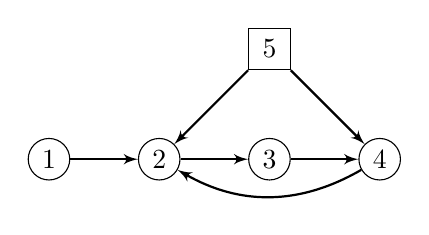
\begin{tikzpicture}[scale=0.7]
			\tikzset{vertex/.style = {shape=circle,draw,minimum size=1.5em, 
			inner 
					sep = 0pt}}
			\tikzset{edge/.style = {->,> = latex', thick}}
			\tikzset{edgebi/.style = {<->,> = latex', thick}}
			\tikzset{every loop/.style={min distance=8mm, looseness=5}}
			\tikzset{vertexFac/.style = {shape=rectangle,draw,minimum 
			size=1.5em, 
					inner sep = 0pt}}
			
			% vertices
			%\draw [line width=35pt,opacity=0.1, blue,line cap=round,rounded
			%corners] (0,0.5) -- (0,2) -- (-1.5,1.5) -- (0,0.5);
			\node[vertex] (a) at  (-4,0) {$1$};
			\node[vertex] (b) at  (-2,0) {$2$};
			\node[vertex] (c) at  (0,0) {$3$};
			\node[vertex] (d) at  (2,0) {$4$};
			\node[vertexFac] (e) at  (0,2) {$5$};
			
			%edges
			
			\draw[edge] (a) to (b);
			\draw[edge] (b) to (c);
			\draw[edge] (c) to (d);
			\draw[edge, bend left = 30] (d) to (b);
			\draw[edge] (e) to (d);
			\draw[edge] (e) to (b);
			
			\end{tikzpicture}
		\end{subfigure}
		\begin{subfigure}{0.48\linewidth}
			\centering
			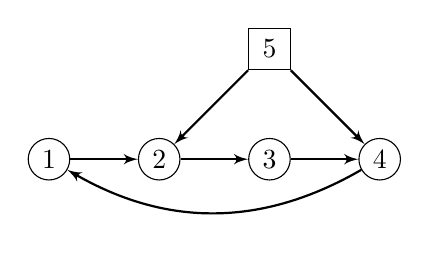
\begin{tikzpicture}[scale=0.7]
			\tikzset{vertex/.style = {shape=circle,draw,minimum size=1.5em, 
					inner 
					sep = 0pt}}
			\tikzset{edge/.style = {->,> = latex', thick}}
			\tikzset{edgebi/.style = {<->,> = latex', thick}}
			\tikzset{every loop/.style={min distance=8mm, looseness=5}}
			\tikzset{vertexFac/.style = {shape=rectangle,draw,minimum 
					size=1.5em, 
					inner sep = 0pt}}
			
			% vertices
			%\draw [line width=35pt,opacity=0.1, blue,line cap=round,rounded
			%corners] (0,0.5) -- (0,2) -- (-1.5,1.5) -- (0,0.5);
			\node[vertex] (a) at  (-4,0) {$1$};
			\node[vertex] (b) at  (-2,0) {$2$};
			\node[vertex] (c) at  (0,0) {$3$};
			\node[vertex] (d) at  (2,0) {$4$};
			\node[vertexFac] (e) at  (0,2) {$5$};
			
			%edges
			
			\draw[edge] (a) to (b);
			\draw[edge] (b) to (c);
			\draw[edge] (c) to (d);
			\draw[edge, bend left = 30] (d) to (a);
			\draw[edge] (e) to (d);
			\draw[edge] (e) to (b);

			
			\end{tikzpicture}
		\end{subfigure}
		%\end{tabular}
		\caption{\label{fig:cyclicDGs} Loops (self-edges) are omitted from this 
		vizualiation. Circles represent observed coordinate processes and 
		squares represent unobserved processes. Left: . Right: }
	\end{figure*}
	
	We consider the graph in Figure \ref{fig:cyclicDGs} (right). When 5 is 
	unobserved, we cannot in general identify any entries of $R$ or of $G$ from 
	the integrated covariances ($C$) [make argument, and find example to show 
	this - what is actually not id'ed? Both R's and G's, or just G's???]. 
	Instead we assume in this example that we also have access to the 
	covariance processes. In this case, the causal functions 
	$g_{11},g_{41},g_{23}$, and $g_{33}$ are identified (Proposition 
	\ref{prop:gPaId}), and therefore so are $G_{11}, G_{41} , G_{23}$ and 
	$G_{33}$.
\end{exmp}

[use/refer here to the general framework of finding additional identification 
using known parameters, see Chen et al.]

[generic identifiability still holds? general result for cyclic models?]

\cite{chenIJCAI2016} and \cite{chenICML2017} describe a framework for 
leveraging prior knowledge of 
model coefficients in linear structural equation models to obtain stronger 
identification results in the acyclic case (see also references in 
\cite{chenICML2017} for earlier applications of similar ideas).


%%%%%%%%%%%%%%%%%%%%%%%%%%%
%%%%%%%%%%%%%%%%%%%%%%%%%%%

\section{Conclusion}

A Hawkes process is defined using the set of $g_{\beta\alpha}$-functions along 
with the $\mu_\alpha$-constants for $\alpha,\beta$ in the finite set $V$. The 
constraints that are shown to exist in this paper are not the only constraints 
imposed by the distribution of the Hawkes process [do I actually know this?] On 
the other hand, they seem to offer also a dimension reduction in that we 
actually test these constraints using a finite parameter space instead of a 
function space. This should make them more suitable to employ in data analysis, 
seeing estimation of $g$ is a challenging problem even in the case of full 
observation [cite recent work] and partial observation only adds to the 
complexity of this task [cite nicolajs thesis]. This approach partially 
circumvents this problem (ref also Achab's paper).


%%%%%%%%%%%%%%%%%%%%%%%%%%%
%%%%%%%%%%%%%%%%%%%%%%%%%%%


\begin{contributions} % will be removed in pdf for initial submission,
                      % so you can already fill it to test with the
                      % ‘accepted’ class option

\end{contributions}

\begin{acknowledgements} % will be removed in pdf for initial submission,
                         % so you can already fill it to test with the
                         % ‘accepted’ class option
    This work was supported by a research grant from
    VILLUM FONDEN (13358).
\end{acknowledgements}

\bibliography{parentalLearning}
\end{document}
